\documentclass[tikz, border=2pt]{standalone}
\usepackage[utf8]{inputenc}
\usepackage[T1]{fontenc}

\usepackage{pgfplots}
\pgfplotsset{compat=newest}
\usepackage{pgfmath}

\definecolor{themeBlue}{RGB}{1, 103, 143}
\definecolor{themeOrange}{RGB}{221, 109, 16}
\definecolor{themeTeal}{RGB}{18, 54, 69}
\definecolor{themeGrey}{RGB}{120, 121, 124}
\definecolor{themePurple}{RGB}{130, 85, 175}
\definecolor{themeGreen}{RGB}{145, 170, 75}

\begin{document}
    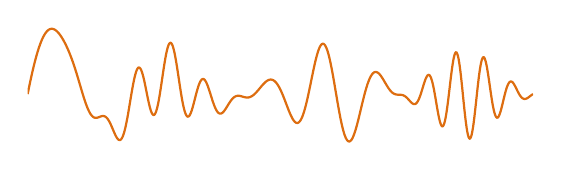
\begin{tikzpicture}
        \begin{axis}[
%            axis lines=middle,
%            xlabel={$t$ [s]},
%            ylabel={Amplitude},
            hide axis,
            xmin=0, xmax=1.5,
            ymin=-1.5, ymax=1.5,
            samples=800,
            domain=0:1.5,
            xtick=\empty,
            ytick=\empty,
            width=8cm,
            height=5cm,
            ]
            \addplot[thick, themeOrange]
            {
                exp(-4*x) * sin(deg(2*pi*3*x)) +
                0.4 * exp(-40*(x-0.4)^2) * sin(deg(2*pi*10*x)) +
                0.6 * exp(-50*(x-0.9)^2) * sin(deg(2*pi*6*x)) +
                0.5 * exp(-70*(x-1.3)^2) * sin(deg(2*pi*12*x))
            };
        \end{axis}
    \end{tikzpicture}
\end{document}